\documentclass[11pt,conference]{IEEEtran}
\IEEEoverridecommandlockouts
\usepackage{amsmath}
\usepackage{amssymb}
\usepackage[english]{babel}
\usepackage{float}
\usepackage[margin=1in]{geometry}
\usepackage[utf8]{inputenc}
\usepackage[square,numbers]{natbib}
\usepackage{tikz}
\usetikzlibrary{automata,positioning}
\pagenumbering{gobble}
\bibliographystyle{plainnat}
\def
\BibTeX{{\rm B\kern-.05em{\sc i\kern-.025em b}\kern-.08em
    T\kern-.1667em\lower.7ex\hbox{E}\kern-.125emX}}
\begin{document}

\title{Publisher/Subscriber Service}

\author{
	\IEEEauthorblockN{Xiao Xin}
	\IEEEauthorblockA{
		\textit{Stanford University} \\
		\textit{xxin@stanford.edu}
	} \\
	\and
	\IEEEauthorblockN{Chi Zhang}
	\IEEEauthorblockA{
		\textit{Stanford University} \\
		\textit{zcdirk@stanford.edu}
	}
}

\maketitle

\begin{abstract}
Publisher/Subscriber (Pub/Sub) is an asynchronous messaging-oriented service that serves as the backbone of contemporary distributed systems. In many cases it is used to decouple the functions of a massive monolithic application by aggregating multiple smaller yet more cohesive services. Being such a critical component to distributed systems, Pub/Sub services should also be scalable so it could fit the requirement of the services that depend on it. This project aims to replicate the functions of a pub/sub service with the capabilities to horizontally scale onto multiple machines to better serve the distributed systems it supports.

\end{abstract}

\section{Overview}
Intuitively, a Pub/Sub system has two components: publisher and subscriber. If a publisher knows what clients are its subscribers, messages will be delivered as requested. However, such design could be troublesome once the number of publishers and subscribers increases, total numbers of connection between publishers and subscribers increases exponentially, which would make the system highly coupled and barely manageable. To resolve the concern, broker, a middleware to decouple relations between publishers and subscribers, is introduced to the system.
	
	\begin{figure}[H]
	\centering
	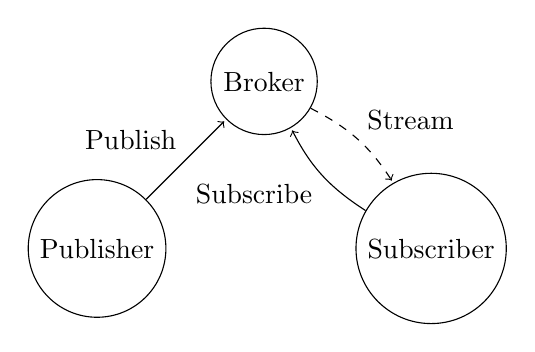
\begin{tikzpicture}[shorten >=1pt,node distance=3cm,on grid,auto]
		\node[state] (0) {Publisher};
		\node[state] (1) [above right=of 0]{Broker};
		\node[state] (2) [below right=of 1]{Subscriber};
		\path[->]
			(0) edge node {Publish} (1)
			(1) edge [bend left=15, dashed] node {Stream} (2)
			(2) edge [bend left=15] node {Subscribe} (1);
	\end{tikzpicture}
	\caption{Pub/Sub System Logical Model}
	\end{figure}

As the figure has shown, with broker in place, publisher and subscribers would only keep track of where the broker is and describe the action it wants to perform to it. The Pub/Sub service designed and implemented in this research serves as the broker in the logic model. It offers the following 2 APIs:

\begin{itemize}
  \item \textbf{Publish}: A client publishes a message of a certain topic to the broker, then the broker will tell the publisher whether the push is completed.
  \item \textbf{Subscribe}: Clients subscribe to topics from the broker, then the broker will push streams of messages under the requested topics to the subscribers.
\end{itemize}

Researchers started off with a primitive monolithic gRPC\citep{grpc} implementation of Pub/Sub on a single machine. Using it as a foundation, the developers then designed sidecar services to assist replication along with single-machine server. For different use cases, Pub/Sub service is implemented to scale up in the following modes:

\begin{itemize}
  \item Master-slave
  \item Leader election using Raft\citep{raft}
\end{itemize}

For each replication mode researchers applied multiple rounds of simulation and load testing using docker-compose\citep{docker-compose}. Each node in the cluster restricted to use 0.5 unit of CPU and 2GB of memory, the cluster is incrementally loaded to host 2000 clients simultaneously, and finally each client is supposed to receive around 20 messages each round and it is supposed to finish receiving all the messages within 1 second. 

The goal of this project is to compare how different replication schemes affects the performance of a distributed Pub/Sub system; hence, for simplicity all implementation only handles storage at memory level, no data is persisted any time in the lifecycle of a server process.


\section{Single-Machine}
The single machine implementation uses a thread-safe map internally to manage topics and subscribers. Each subscriber is put into its own thread\footnote{Service is implemented in Go\citep{golang}, where a thread is a go-routine.}. Every time a message is published, broker will first deliver the message to the subscriber threads of the message topic, and thereafter the message will be transported to clients in each thread. Figure 2 demonstrates the performance of a single-machine service throughout load-testing.

\begin{figure}[H]
	\centering
	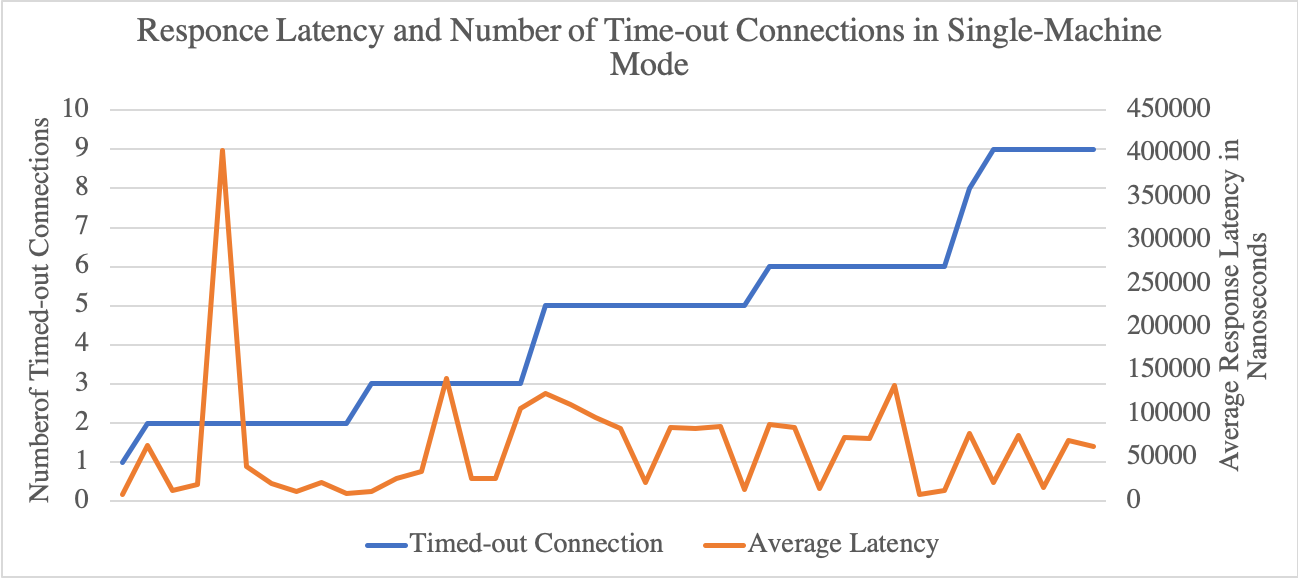
\includegraphics[scale=0.33]{figure/single_machine/performance.png}
	\caption{Single-Machine Performance}
\end{figure}

In average a single-machine service could finish a round of messages within 50 milliseconds. Several clients were blocked in the process and timed out; one possible reason could be that there is only one simulation process, so the client threads were locked, or maybe neglected, during user context switching. The issue should be negligible since the overall time-out rate is less than 0.5\%. The researchers later applied load-testing using the same setup to find out the maximum capacity of this implementation, and statistics showed that such a service could be handle 20000 clients with roughly 3\% timeout rate.

	
\section{Replication}
Although single-machine implementation could achieve acceptable performance, its capacity upper-bound is strictly limited by the computing power and storage space of the machine hosting it, and one must upgrade the hosting machine to scale up, which could be rather expensive. Following implementations provides ways to scale up the overall service capacities of the system by replicating and coordinating service process onto multiple machines. The machines involved in a distributed Pub/Sub systems are called \textbf{nodes}, and all nodes form a \textbf{cluster} that implements the functions of Pub/Sub systems.


\subsection{Master-Slave}
In master-slave cluster, a node is either a \textbf{master} or a \textbf{slave}. There is one and only one master in a cluster; master has no master to itself but slaves always have either a master or another slave as its master. Together all these nodes forms a tree-like topology with the root of the tree being the master of the cluster. 

In this mode each node has a sidecar service to assist master-slave replication.  Upon initiation, slaves post a request to its master's sidecar service to register as a known slave.

Masters and slaves handles subscribe action just as single machine implementation. Therefore, the system could easily increase reading throughput linearly by adding more nodes into the cluster. 

For publish, a slave would propagate the message to its master until the master of the cluster. Once received the message, the master would broadcast the message to all its slaves through their master-slave sidecar service, and then perform a publish action to its subscribers same as single-machine service. For slaves, they each manages a thread to listen to confirmed publish messages from its master, publish the message to its subscribers, and keep relaying the message to its slaves.

Since master-slave cluster forms a tree, one of the proposed design is to let nodes reserve a special topic for its slaves, and the slaves can just subscribe to the special topic to relay messages to their subscribers. However, the implementation is not adapted eventually for two reasons: first, developers have to introduce a guarding scheme to prevent users from interrupting system messages in reserved topics; second, the messages in reserved topic will have to be serialized at master to include metadata such as topic name and then deserialized at slaves, which introduces unnecessary operations. 

\begin{figure}[H]
	\centering
	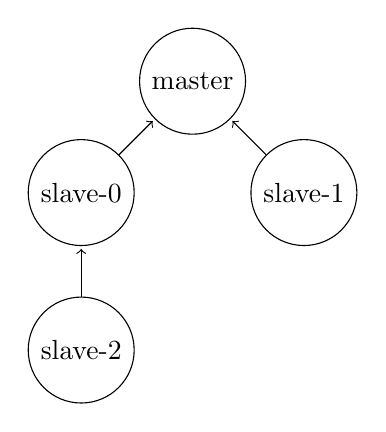
\begin{tikzpicture}[shorten >=1pt,node distance=2cm,on grid,auto]
		\node[state] (0) {master};
		\node[state] (1) [below left=of 0]{slave-0};
		\node[state] (2) [below right=of 0]{slave-1};
		\node[state] (3) [below=of 1]{slave-2};
		\path[->]
			(1) edge node {} (0)
			(2) edge node {} (0)
			(3) edge node {} (1);
	\end{tikzpicture}
	\caption{Master-Slave Cluster Topology}
\end{figure}
	
The researchers set up a cluster with 4 nodes organized as figure 4 for load testing. This organization includes all potential master-slave relation that could exists in master-slave mode, which could provide a more comprehensive demonstration of cluster performance.
	
\begin{figure}[H]
	\centering
	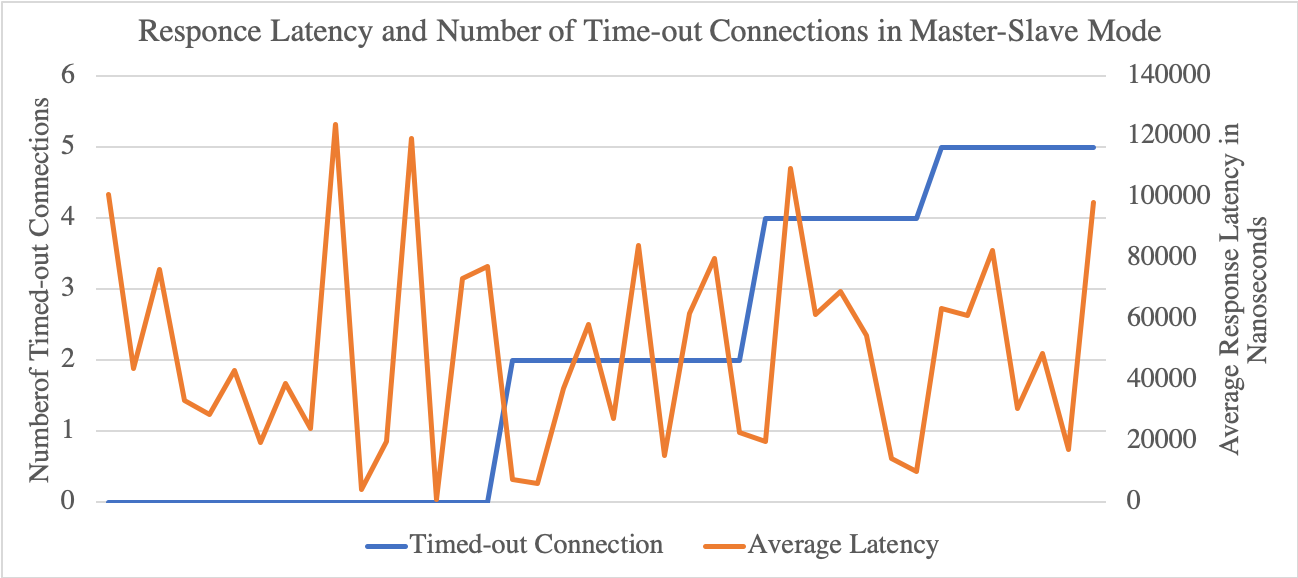
\includegraphics[scale=0.33]{figure/master-slave/performance.png}
	\caption{Master-Slave Performance}
\end{figure}

\begin{figure}[H]
	\centering
	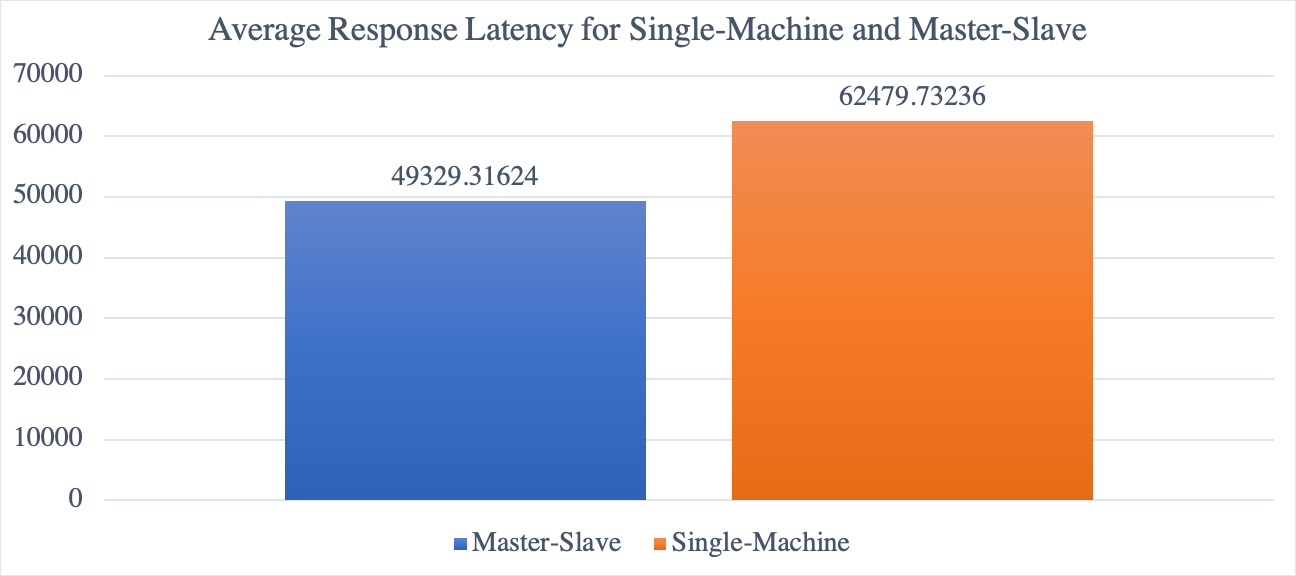
\includegraphics[scale=0.33]{figure/master-slave/response-latency.png}
	\caption{Single-Machine/Master-Slave average response latency}
\end{figure}

Figure 5 and 6 provide an overview of the capacity of master-slave Pub/Sub cluster. The statistics reflects here that, comparing to single-machine implementation, master-slave is slightly faster and has fewer timed out connections throughout the testing process. The testing program evenly distributed clients among nodes in the cluster, therefore causing each node  to handle only a quarter of load using the same amount of resources as the single-machine instance. The researchers actually expected master-slave architecture to be slower due to potential latency that may caused by message propagation through network. But since the testing cluster is hosted as containers sharing a virtual network on a single machine, the effect of network latency appears to become negligible. This finding could be helpful to users when they apply Pub/Sub in production, as they might be able to use master-slave mode to dispatch or collect data rapidly across regions with the leverage of reliable and performant network service, such as Google Could's high-performance premium tier network solution\citep{google-cloud-network}.

Master-slave's demonstrate decent potential, but its performance is in trade of reliability. If one node were to go down, all of the node's slaves and sub-slaves will lost sync with the rest the cluster at the same time. Besides, a master-slave cluster's performance is strongly correlated to its topology. If the cluster tree is too deep, or some of the nodes serving too many clients, the cluster's performance could be significantly affected. Only a balanced-tree of reasonable height with clients evenly distributed among nodes would make the cluster perform the finest. 
\

\subsection{Raft}
Raft mode provides a less performant yet more reliable replication scheme for Pub/Sub. In master-slave mode

\begin{figure}[H]
	\centering
	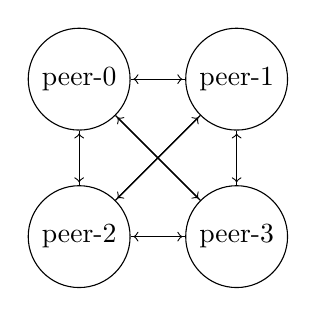
\begin{tikzpicture}[shorten >=1pt,node distance=2cm,on grid,auto]
		\node[state] (0) {peer-0};
		\node[state] (1) [right=of 0]{peer-1};
		\node[state] (2) [below=of 0]{peer-2};
		\node[state] (3) [right=of 2]{peer-3};
		\path[->]
			(0) edge node {} (1)
			(0) edge node {} (2)
			(0) edge node {} (3)
			
			(1) edge node {} (0)
			(1) edge node {} (2)
			(1) edge node {} (3)
			
			
			(2) edge node {} (0)
			(2) edge node {} (1)
			(2) edge node {} (3)
			
			
			(3) edge node {} (0)
			(3) edge node {} (1)
			(3) edge node {} (2);
	\end{tikzpicture}
	\caption{Raft Cluster Topology}
\end{figure}
	
\begin{figure}[H]
	\centering
	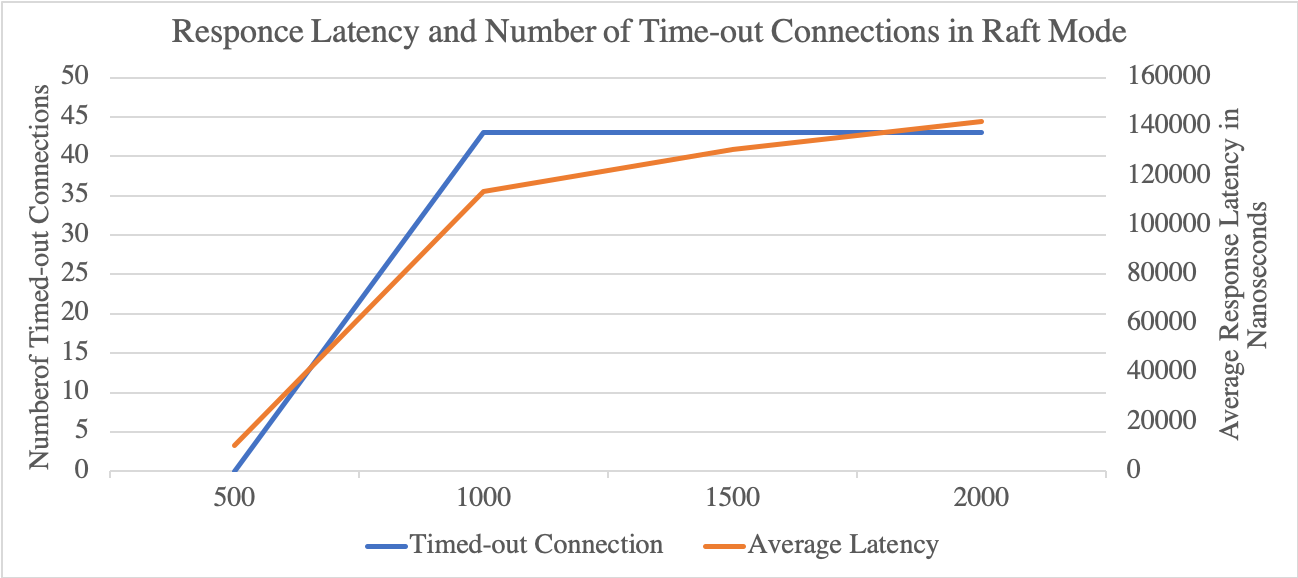
\includegraphics[scale=0.33]{figure/raft/performance.png}
	\caption{Raft Performance}
\end{figure}
	
\begin{figure}[H]
	\centering
	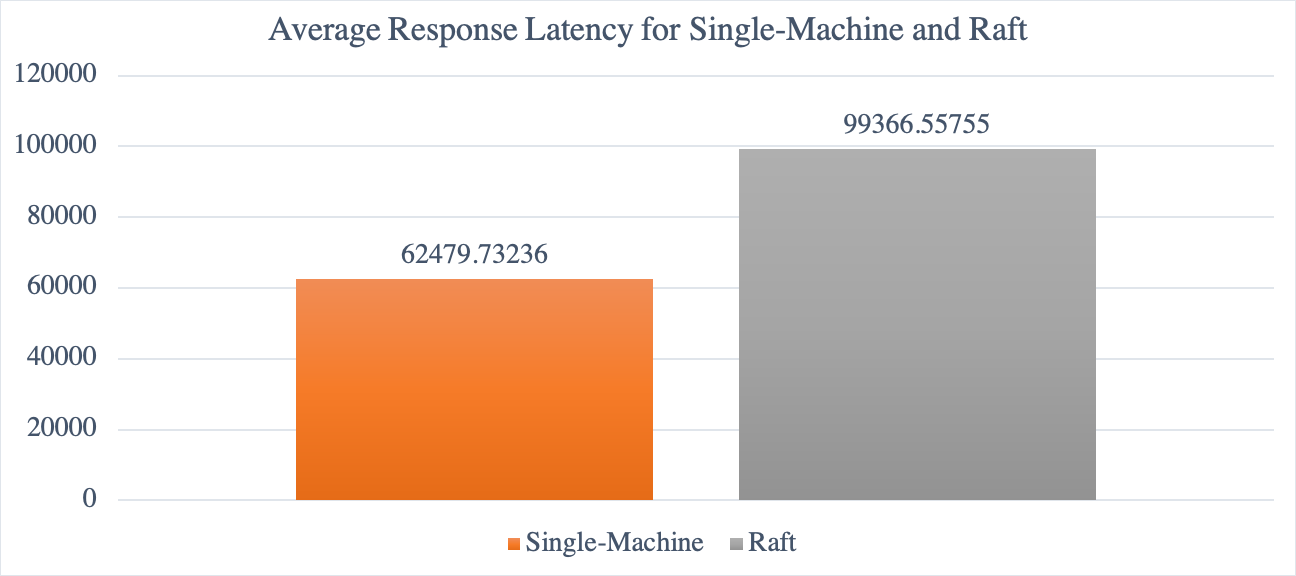
\includegraphics[scale=0.33]{figure/raft/response_latency.png}
	\caption{Single-Machine/Raft average response latency}
\end{figure}

% TODO (zcdirk@)
% Talk about optimization strategies in Raft implementation


\section{Conclusion}
Scaling remains one of the hardest problem in computer science and software engineering. Through this project, the researchers learned that different scaling approaches has its own comparative advantages: master-slave architecture could be one way to extend system performance; meanwhile leader election could be another way to improve system reliability. However, learning the advantages is not yet enough, the researchers also developed some thinking on how Pub/Sub and scaling could be further optimized in future.

First, the testing strategy adapted throughout the research mostly focused on subscribing side. Subscribe have to keep a long-lasting socket with Pub/Sub servers, but publish is more of a short-lived request but could take place frequently. Given current architectures, where all publish requests are essentially routed to a leader machine, when the publish traffic is at high level the performance of the system could be very different. Hence, how to scale up publish requests still remains an interesting problem that can be better addressed.

Second, after this project the researchers have the idea that the future of scaling solutions should be hybrid of multiple approaches. The essence of a distributed system is the topology it forms; therefore the system users should be able to manipulate such structure however they want to most efficiently solve the problems they need to tackle. Hence, if a distributed system solution could be configured to easily adapt multiple replication strategies, it is likely to be preferred by more users. While developing this system, the researchers attempted to extract the scaling functions as a set of standard interfaces, and the side-car services could just implement the interface. If this goal were to be achieved, the Pub/Sub system the researchers have designed could be able to provide multiple means of replication strategies on a single node. But this idea was eventually unapproachable due to the fact that Pub/Sub implementation needs to be written, such as rerouting publish requests to masters, in different replication strategies so that the strategy could work. In order to achieve the proposed idea, the Pub/Sub base API should be better designed so it has the flexibility to fit the requirements of replication strategies.

% TODO (zcdirk@)
% Talk about future action items 

\medskip
\bibliography{references}

\end{document}
